\documentclass{beamer}

\usepackage{beamerthemesplit}
\usepackage{verbatim}
\usepackage[normalem]{ulem}

\usepackage{xcolor}

\usepackage{hyperref}

\definecolor{gold}{rgb}{1.,0.84,0.}
\definecolor{brightred}{rgb}{1.,0.4,0.4}
\definecolor{mygray}{RGB}{200,200,200}
\definecolor{lightsteelblue}{RGB}{176,196,222}
\definecolor{lightskyblue}{RGB}{135,206,250}
\definecolor{cadetblue}{RGB}{95,158,160}

\usetheme{default}
\usecolortheme{mule}

\usefonttheme{serif}

%\DeclareGraphicsExtensions{.pdf,.png,.jpg}

\newcommand{\mcal}{\textsc{metacalibration}}
\newcommand{\Mcal}{\textsc{Metacalibration}}

\newcommand{\mcalR}{\mbox{\boldmath $R$}}
\newcommand{\mcalRscalar}{\mbox{$R$}}

\newcommand{\mcalRmean}{\mbox{\boldmath $\langle R \rangle$}}
\newcommand{\mcalRscalarmean}{\mbox{$\langle R \rangle$}}

\newcommand{\mcalRpsf}{$R^{p}$}
\newcommand{\mcalRpsfnoise}{$R^{p}_\eta$}
\newcommand{\mcalRo}{\mbox{\boldmath $R_o$}}
\newcommand{\mcalRnoise}{\mbox{\boldmath $R_\eta$}}

\newcommand{\mcalRmeanalpha}{\mbox{\boldmath $\langle R_\alpha \rangle$}}
\newcommand{\mcalRmeanbeta}{\mbox{\boldmath $\langle R_\beta \rangle$}}

\newcommand{\mcalRg}{\mbox{\boldmath $R_\gamma$}}
\newcommand{\mcalRS}{\mbox{\boldmath $R_S$}}
\newcommand{\mcalRgmean}{\mbox{\boldmath $\langle R_\gamma \rangle$}}
\newcommand{\mcalRSmean}{\mbox{\boldmath $\langle R_S \rangle$}}

\newcommand{\mcalRtwopt}{\mbox{\boldmath $R^{2pt}$}}
\newcommand{\mcalRtwoptmean}{\mbox{\boldmath $\langle R^{2pt} \rangle$}}


\newcommand{\mcalRmodel}{\mbox{\boldmath $R^{model}$}}
\newcommand{\mcalRnoisemodel}{\mbox{\boldmath $R^{model}_\eta$}}


\newcommand{\vecg}{\mbox{\boldmath $\gamma$}}
\newcommand{\vest}{\mbox{\boldmath $e$}}

\newcommand{\snr}{$S/N$}
\newcommand{\snT}{$(S/N)_{\textrm{size}}$}
%\newcommand{\snT}{$\left( \frac{S}{N}\right)_{\textrm{size}}$}
\newcommand{\snflux}{$(S/N)_{\textrm{flux}}$}
%\newcommand{\snflux}{$\left( \frac{S}{N}\right)_{\textrm{flux}}$}

\newcommand{\lensfit}{\texttt{LENSFIT}}
\newcommand{\numba}{\texttt{Numba}}
\newcommand{\python}{\texttt{Python}}
\newcommand{\ngmix}{\texttt{ngmix}}
\newcommand{\shear}{{\bf g}}
\newcommand{\redmapper}{redMaPPer}
\newcommand{\est}{$e$}


\newcommand{\prelim}{{\bf{\it Preliminary}}}

\newcommand{\uberseg}{{\"u}berseg}


\title{\mcal\ for Weak Lensing Sheare Estimation \\
or\\
Metacal Don't Care}
\author{Erin Sheldon}
\institute{Brookhaven National Laboratory}

% http://texblog.net/latex-archive/plaintex/beamer-footline-frame-number/
% to add the page (frame ) number and not screw up the bottom line
% works for split themes?
\expandafter\def\expandafter\insertshorttitle\expandafter{%
      \insertshorttitle\hfill%
        \insertframenumber\,/\,\inserttotalframenumber}

% suppress navigation bar
\beamertemplatenavigationsymbolsempty
\setbeamertemplate{footline}{}

\begin{document}

\frame{\titlepage}


\setbeamertemplate{background canvas}[vertical shading][bottom=mgray,top=mblack]

\frame
{
    \frametitle{Outline}

    \setbeamerfont*{itemize/enumerate body}{size=\Large}
    \setbeamerfont*{itemize/enumerate subbody}{parent=itemize/enumerate body}
    \setbeamerfont*{itemize/enumerate subsubbody}{parent=itemize/enumerate body}
 
    \begin{itemize}

        \item Introduction to \mcal
        \item Performance on Simulations

    \end{itemize}

}

\frame
{
    \frametitle{Shear Accuracy Requirements}

    \setbeamerfont*{itemize/enumerate body}{size=\Large}
    \setbeamerfont*{itemize/enumerate subbody}{parent=itemize/enumerate body}
    \setbeamerfont*{itemize/enumerate subsubbody}{parent=itemize/enumerate body}
 
    \begin{itemize}

        \item In order to measure the Dark Energy equation of state
            to the desired accuracy for LSST, we must measure
            shear with exquisite accuracy.

            {\color{lightskyblue}
                \begin{equation}
                    \gamma = (1 + m ) \times \gamma_{true} + c \nonumber
                \end{equation}
            } 

        \item LSST Requirements
            \begin{itemize}
                \item Multiplicative errors: {\color{gold} $m \lesssim 0.001$}
                \item Additive errors: {\color{brightred} $c \lesssim 0.0001$}
            \end{itemize}


    \end{itemize}

}

\frame
{
    \frametitle{Sources of Systematic Error in Typical Estimators}

    \setbeamerfont*{itemize/enumerate body}{size=\large}
    \setbeamerfont*{itemize/enumerate subbody}{parent=itemize/enumerate body}
    \setbeamerfont*{itemize/enumerate subsubbody}{parent=itemize/enumerate body}
 
    \begin{itemize}

        \item Galaxy models used to infer ellipticity and shear 
            typically wildly inaccurate, error exceeds budget.

        \item Noise biases shape determination, exceed error budget.

        \item Most of the galaxies in ground based surveys are
            unresolved, worsening modeling and noise effects.

        \item Selection effects can easily exceed error budget.

        \item Effects of neighbors and undetected objects can cause
            large bias, especially when calibrating from sims.

        \item PSF Modeling must be accurate (effects {\em all} known estimators)

    \end{itemize}

}


\frame
{
    \frametitle{\Mcal}

    \setbeamerfont*{itemize/enumerate body}{size=\Large}
    \setbeamerfont*{itemize/enumerate subbody}{parent=itemize/enumerate body}
    \setbeamerfont*{itemize/enumerate subsubbody}{parent=itemize/enumerate body}
 
 \begin{itemize}
     \item Designed to correct for noise bias, model bias, selection bias.
     \item No reliance on simulations or significant prior information
         for basic shear calibration.
 \end{itemize}

}

\frame
{
    \frametitle{\Mcal\ Idea from Eric Huff (Kaiser)}

    \setbeamerfont*{itemize/enumerate body}{size=\large}
    \setbeamerfont*{itemize/enumerate subbody}{parent=itemize/enumerate body}
    \setbeamerfont*{itemize/enumerate subsubbody}{parent=itemize/enumerate body}
 
    \begin{itemize}

        \item Suppose we have a biased shear estimator {\color{gold} \vest}.  Then we can write
            {\color{gold}
\begin{align} \label{eq:Eexpand}
    \vest &= \vest|_{\gamma=0} + \frac{ \partial \vest }{ \partial \vecg}\bigg|_{\gamma=0} \vecg  + ... \nonumber \\
          &\equiv \vest|_{\gamma=0} + \mbox{\mcalR}\vecg  + ...
\end{align}
            } 

        \item For an ensemble mean
            {\color{gold}
                \begin{align}
                    \langle \vest \rangle &= \langle \vest \rangle |_{\gamma=0} + \langle \mbox{\mcalR} \vecg \rangle + ... \nonumber \\
                                          &\approx \langle \mbox{\mcalR} \vecg \rangle,
                \end{align}
                }

            \item The shear is weighted by responses {\color{cadetblue} \mcalR}.  If we know the
                responses, we can form a weighted average:
            {\color{gold}
\begin{align} \label{eq:rcorr}
    \langle \vecg \rangle &\approx \langle \mbox{\mcalR} \rangle^{-1}  \langle \vest \rangle \approx \langle \mbox{\mcalR} \rangle^{-1} \langle \mcalR \vecg \rangle.
\end{align}
            }
    \end{itemize}
}

\frame
{
    \setbeamerfont*{itemize/enumerate body}{size=\Large}
    \setbeamerfont*{itemize/enumerate subbody}{parent=itemize/enumerate body}
    \setbeamerfont*{itemize/enumerate subsubbody}{parent=itemize/enumerate body}
 
    \frametitle{Numerical Derivative}

       \begin{itemize}

        \item Use image manipulation to estimate the derivative of the
            estimator with respect to shear
            {\color{gold}
                \begin{equation}
                    \mcalR = \frac{\vest^+ - \vest^-}{\Delta \vecg} \nonumber 
                \end{equation}
            }
            \begin{itemize}
                \item Deconvolve the PSF
                \item Shear the image by a small amount
                \item Reconvolve by a new function.  Should be larger than PSF to suppress
                    noise amplification. 
                \item {\color{lightsteelblue} Add noise field to cancel correlated noise}
            \end{itemize}


    \end{itemize}

}

\frame
{
    \frametitle{Correlated Noise}

    \setbeamerfont*{itemize/enumerate body}{size=\Large}
    \setbeamerfont*{itemize/enumerate subbody}{parent=itemize/enumerate body}
    \setbeamerfont*{itemize/enumerate subsubbody}{parent=itemize/enumerate body}
 

    \begin{itemize}

        \item Convolutions and shearing result in correlated noise.

        \item At \snr$\sim 10$ can cause a 10\% shear bias.

        \item Add a noise field that has been run through the same
            operations, and then rotated by 90 degrees.

        \item Cancels all correlated noise effects at the cost of
            increasing the noise in the shear recovery by 20\% (less
            than $\sqrt 2$ because shape noise dominates).

    \end{itemize}

}



\frame
{
    \frametitle{Selection Effects}

    \setbeamerfont*{itemize/enumerate body}{size=\Large}
    \setbeamerfont*{itemize/enumerate subbody}{parent=itemize/enumerate body}
    \setbeamerfont*{itemize/enumerate subsubbody}{parent=itemize/enumerate body}
 

    \begin{itemize}

        \item  Applying a selection to objects can indirectly select on the shapes
            of galaxies and result in a biased shear measurement.

        \item For example, putting a threshold on \snr\ tends to select less
            elliptical galaxies.

        \item Cannot be ignored: this is a percent level effect.

    \end{itemize}

}

\frame
{
    \frametitle{Selection Effects}

    \setbeamerfont*{itemize/enumerate body}{size=\large}
    \setbeamerfont*{itemize/enumerate subbody}{parent=itemize/enumerate body}
    \setbeamerfont*{itemize/enumerate subsubbody}{parent=itemize/enumerate body}
 
    \begin{itemize}

        \item If we have a selection function $S$ that has some dependence
            on ellipticity, then the mean ellipticity
            can be biased

            \begin{align}
                {\color{gold} \langle \vest \rangle^S = \int S(\vest)~P(\vest)~\vest~d\vest},
            \end{align}


        \item We can also use quantities measured from sheared images
            to correct for selections. 

            \begin{align}
                \frac{\partial \langle \vest \rangle}{\partial \gamma}\bigg|_{\gamma=0} &\approx
                \frac{\langle \vest^+ \rangle^S - \langle \vest^- \rangle^S}{\Delta \gamma} + \frac{\langle \vest \rangle^{S+} - \langle \vest \rangle^{S-}}{\Delta \gamma} \nonumber \\
                &\equiv {\color{gold} \langle \mcalRg \rangle + \langle \mcalRS \rangle},
            \end{align}

            Where {\color{lightsteelblue} $\langle \vest \rangle^{S+}$}
            represents the mean shape from unsheared images, with selection
            based on parameters measured from
            positively sheared images.

    \end{itemize}

}

\frame
{

    \frametitle{Simulation Tests}


    \begin{itemize}
        \item Galsim
        \item Flux/size drawn jointly from COSMOS 25.2 sample
        \item $S/N$ down to 2.
        \item Bulge+Disk with different ellipticities.
        \item Knots of star formation (\texttt{galsim.RandomWalk})
        \item Apply threshold of $5-\sigma$ {\em before} \mcal, so this
            mimics detection thresholds for which we cannot correct.
        \item PSF Moffat $e=0.05$, FWHM = 0.9 arcsec.
    \end{itemize}

    (Focus on challenging parametric sim; we also ran on a less challenging 
    ``real-galaxy, realistic PSF'' sim using COSMOS galaxy images.)

}

{

    %\setbeamertemplate{background canvas}[vertical shading][bottom=white,top=white]
    \frame
    {
        \frametitle{Example Galaxies}
     
        {\small Large examples to show internal structure:  actual simulation
        galaxies are almost all smaller than the PSF }

        \begin{center}
            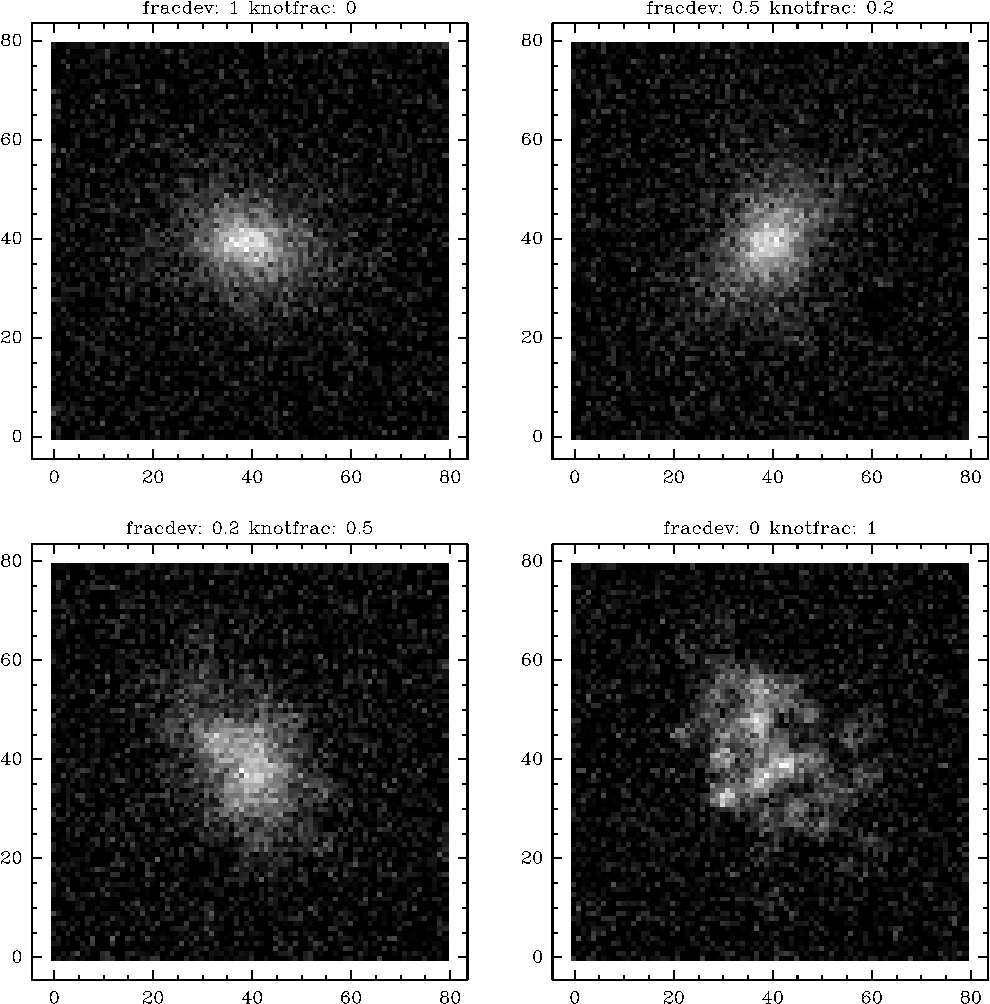
\includegraphics[width=0.7\textwidth]{mosaic-009086.pdf}
            \newline
        \end{center}

    }
    %\setbeamertemplate{background canvas}[vertical shading][bottom=mgray,top=mblack]


}



\frame
{
    \frametitle{\snr}
 
    \begin{center}
        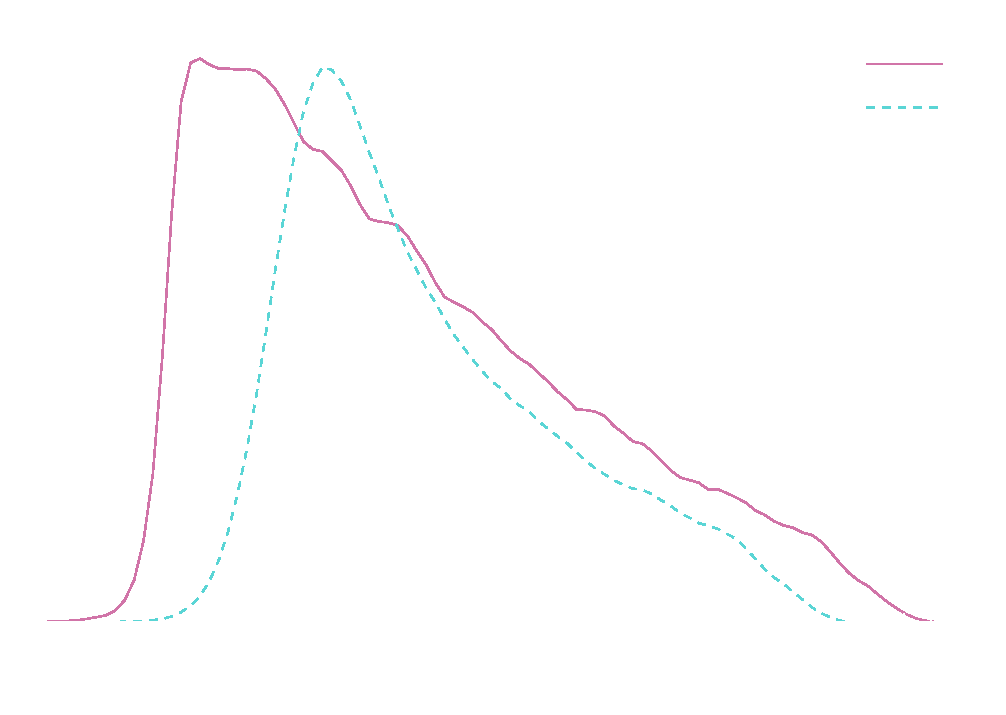
\includegraphics[width=\textwidth]{run-bdj03mcal01-s2n-inv.pdf}
        \newline
    \end{center}



}

\frame
{
    \frametitle{$r_{50}$}
 
    \begin{center}
        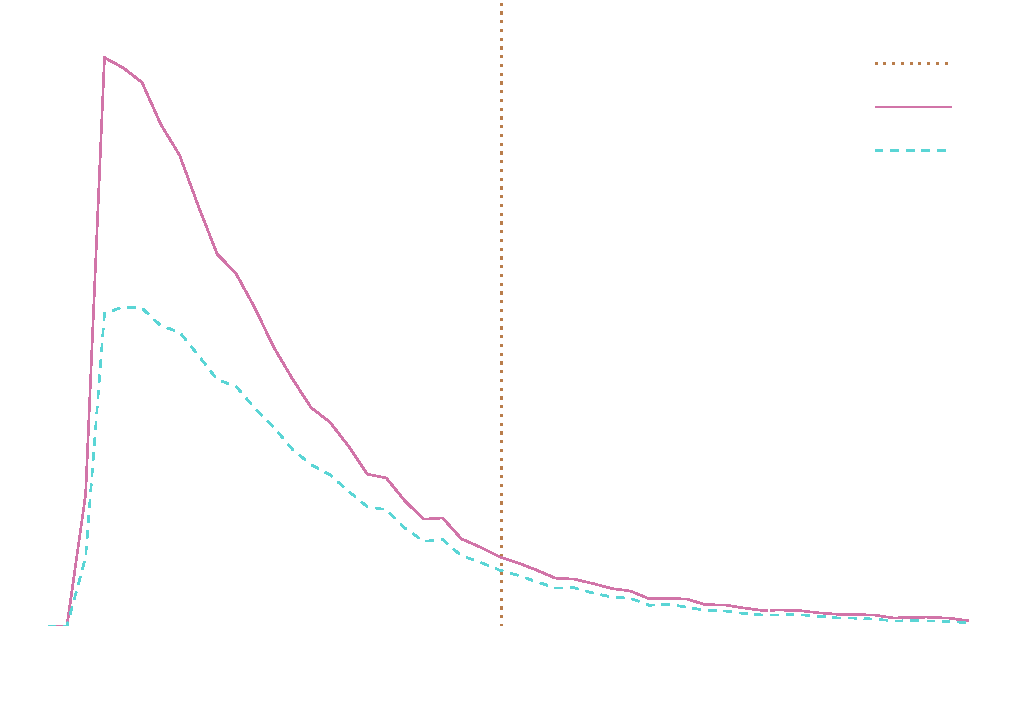
\includegraphics[width=\textwidth]{run-bdj03mcal01-r50-inv.pdf}
        \newline
    \end{center}



}

\frame
{
    \frametitle{Can't Model Galaxies?  Metacal Don't Care}
 
    \setbeamerfont*{itemize/enumerate body}{size=\large}
    \setbeamerfont*{itemize/enumerate subbody}{parent=itemize/enumerate body}
    \setbeamerfont*{itemize/enumerate subsubbody}{parent=itemize/enumerate body}
 
    \begin{columns}
        \begin{column}{0.5\textwidth}
            \begin{itemize}
                \item Fitting {\color{lightsteelblue} adaptive moments} with 
                    {\color{red} no PSF correction}
                \item \snr$ > 10$
                \item {\color{gold}$m = (0.03 \pm 0.31) \times 10^{-3}$}
            \end{itemize}
        \end{column}
        \begin{column}{0.5\textwidth}
            \begin{center}
                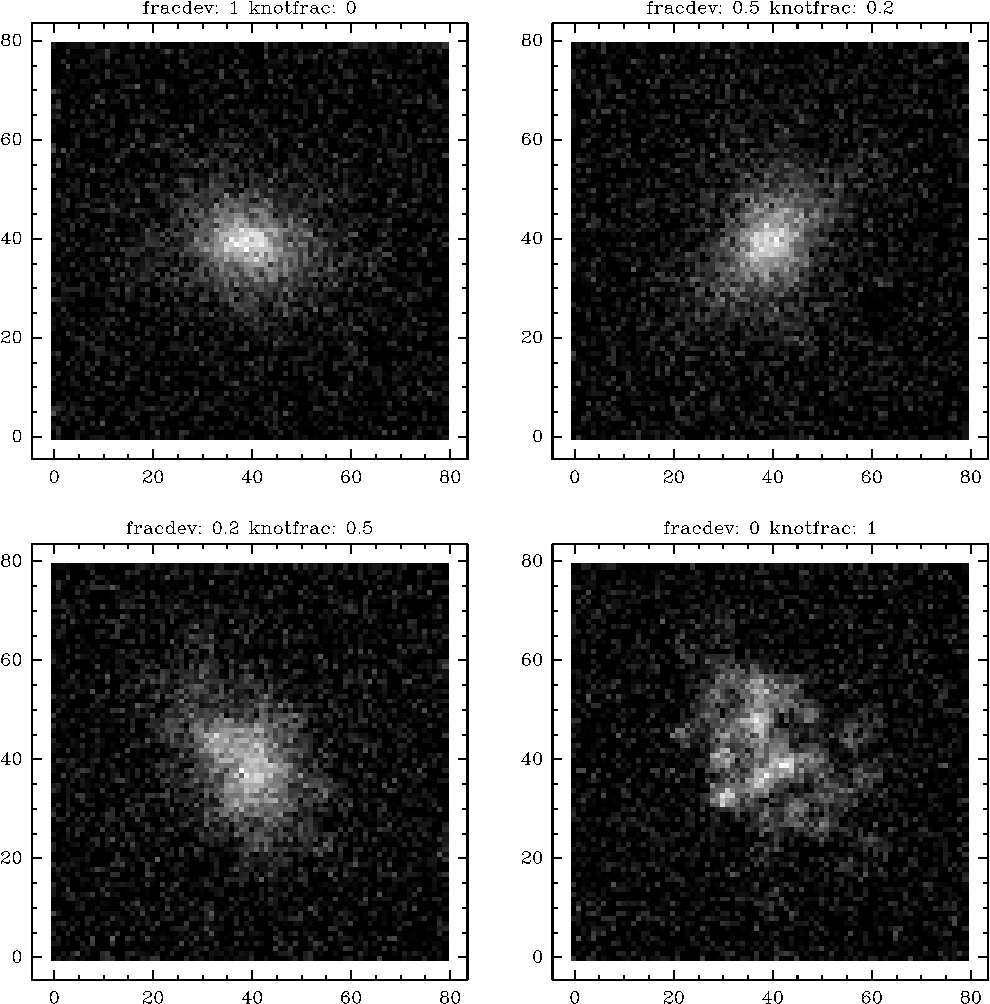
\includegraphics[width=\columnwidth]{mosaic-009086.pdf}
                \newline
            \end{center}
        \end{column}
    \end{columns}


}

\frame
{
    \frametitle{Galaxies Unresolved?  Metacal Don't Care}
 
    \setbeamerfont*{itemize/enumerate body}{size=\large}
    \setbeamerfont*{itemize/enumerate subbody}{parent=itemize/enumerate body}
    \setbeamerfont*{itemize/enumerate subsubbody}{parent=itemize/enumerate body}
 
    \begin{columns}
        \begin{column}{0.5\textwidth}
            \begin{itemize}
                \item No cuts on size.
                \item \snr$ > 10$
                \item {\color{gold}$m = (0.03 \pm 0.31) \times 10^{-3}$}
            \end{itemize}
        \end{column}
        \begin{column}{0.5\textwidth}
            \begin{center}
                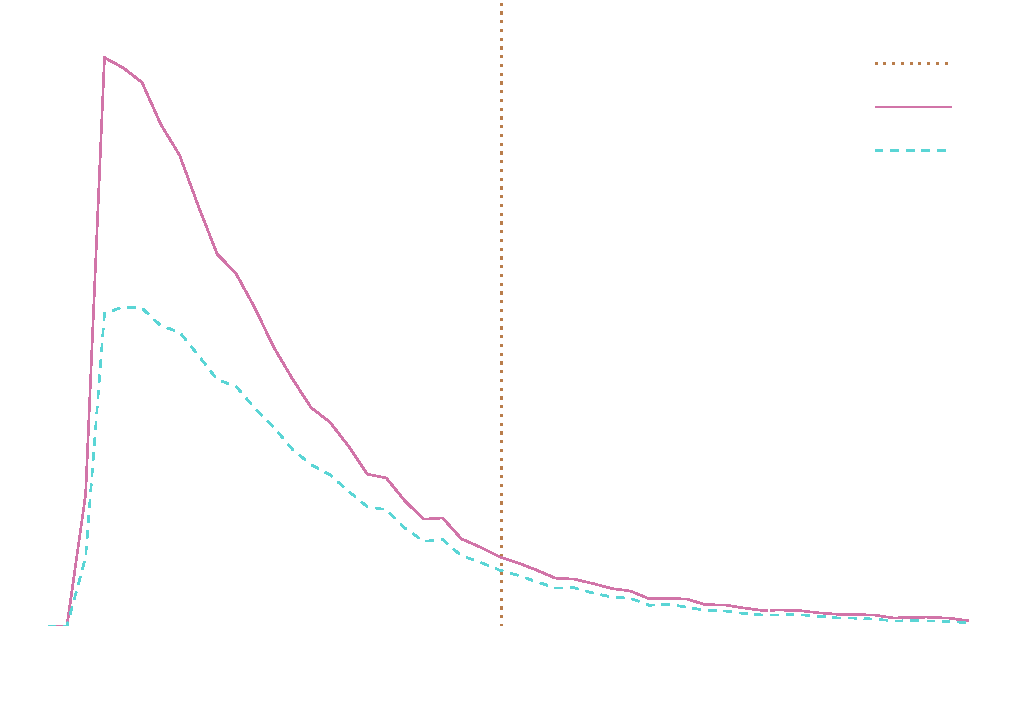
\includegraphics[width=\columnwidth]{run-bdj03mcal01-r50-inv.pdf}
                \newline
            \end{center}
        \end{column}
    \end{columns}


}


\frame
{
    \frametitle{Got No Signal?  Metacal Don't Care}
 
    \setbeamerfont*{itemize/enumerate body}{size=\large}
    \setbeamerfont*{itemize/enumerate subbody}{parent=itemize/enumerate body}
    \setbeamerfont*{itemize/enumerate subsubbody}{parent=itemize/enumerate body}
 
    \begin{columns}
        \begin{column}{0.5\textwidth}
            \begin{itemize}
                \item Push down to  \snr$ > 7$
                \item {\color{gold}$m = (0.55 \pm 0.34) \times 10^{-3}$}
            \end{itemize}
        \end{column}
        \begin{column}{0.5\textwidth}
            \begin{center}
                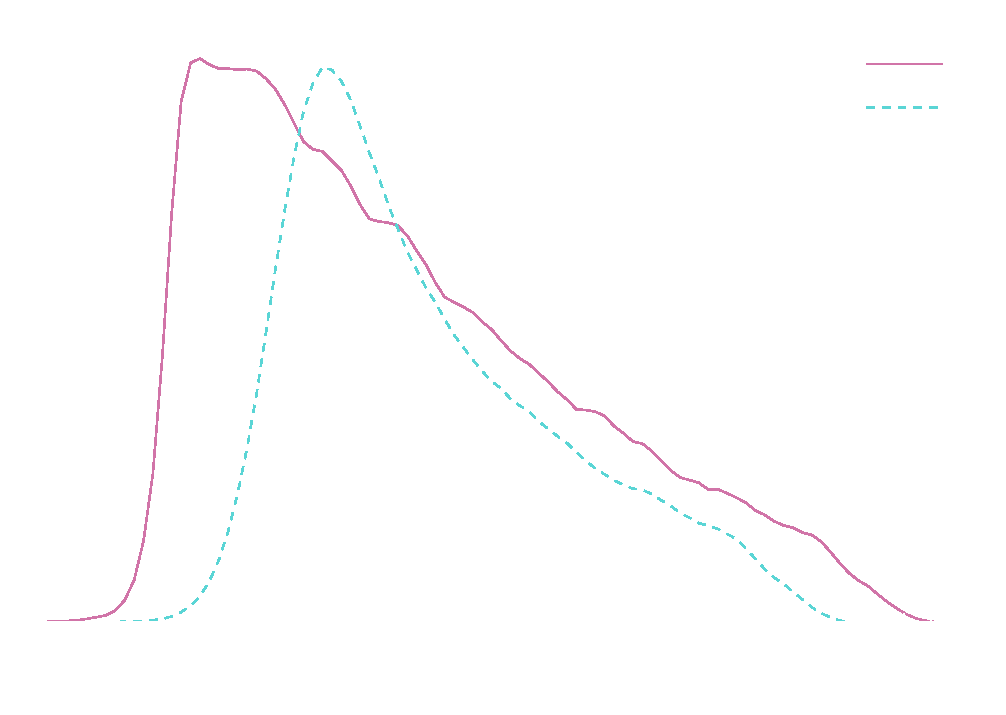
\includegraphics[width=\columnwidth]{run-bdj03mcal01-s2n-inv.pdf}
                \newline
            \end{center}
        \end{column}
    \end{columns}


}


\frame
{
    \frametitle{Don't Know What You're Doing?  Metacal Don't Care}
 
    \setbeamerfont*{itemize/enumerate body}{size=\large}
    \setbeamerfont*{itemize/enumerate subbody}{parent=itemize/enumerate body}
    \setbeamerfont*{itemize/enumerate subsubbody}{parent=itemize/enumerate body}
 
    \begin{columns}
        \begin{column}{0.4\textwidth}
            \begin{itemize}
                \item Naively cut on {\color{lightsteelblue} \snr}, which correlates
                    strongly with ellipticity.
                \item The formalism corrects your mistake.
            \end{itemize}
        \end{column}
        \begin{column}{0.6\textwidth}
            \begin{center}
            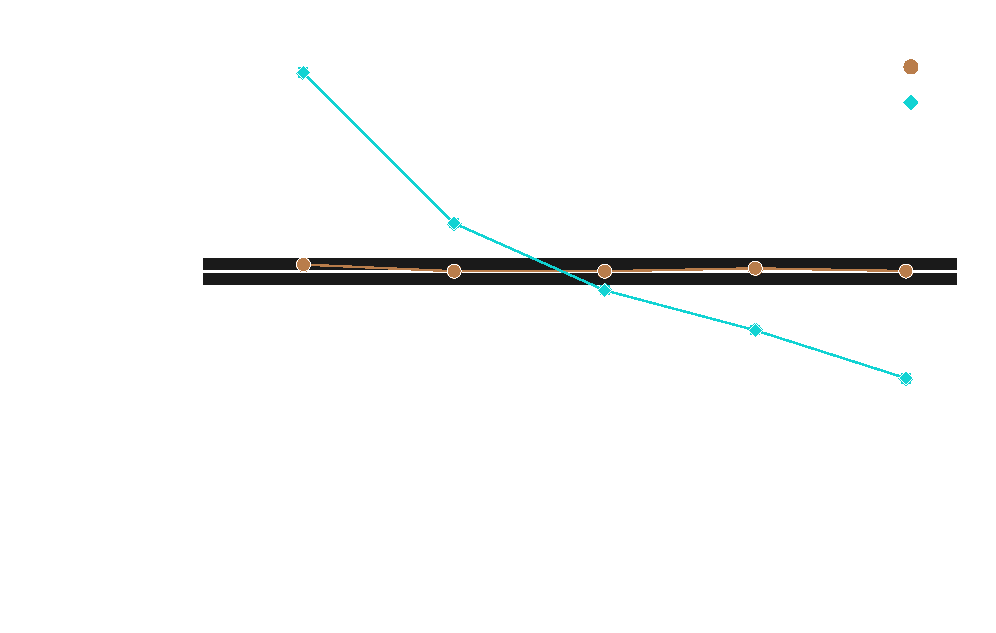
\includegraphics[width=\textwidth]{mc-select-bias-thresh-with-nocorr-inv.pdf}
                \newline
            \end{center}
        \end{column}
    \end{columns}


}



\frame
{
    \frametitle{Don't Know What You're Doing?  Metacal Don't Care}
 
    \setbeamerfont*{itemize/enumerate body}{size=\large}
    \setbeamerfont*{itemize/enumerate subbody}{parent=itemize/enumerate body}
    \setbeamerfont*{itemize/enumerate subsubbody}{parent=itemize/enumerate body}
 
    \begin{columns}
        \begin{column}{0.4\textwidth}
            \begin{itemize}
                \item Naively cut on {\color{lightsteelblue} \snr}, which correlates
                    strongly with ellipticity.
                \item The formalism corrects your mistake.
            \end{itemize}
        \end{column}
        \begin{column}{0.6\textwidth}
            \begin{center}
            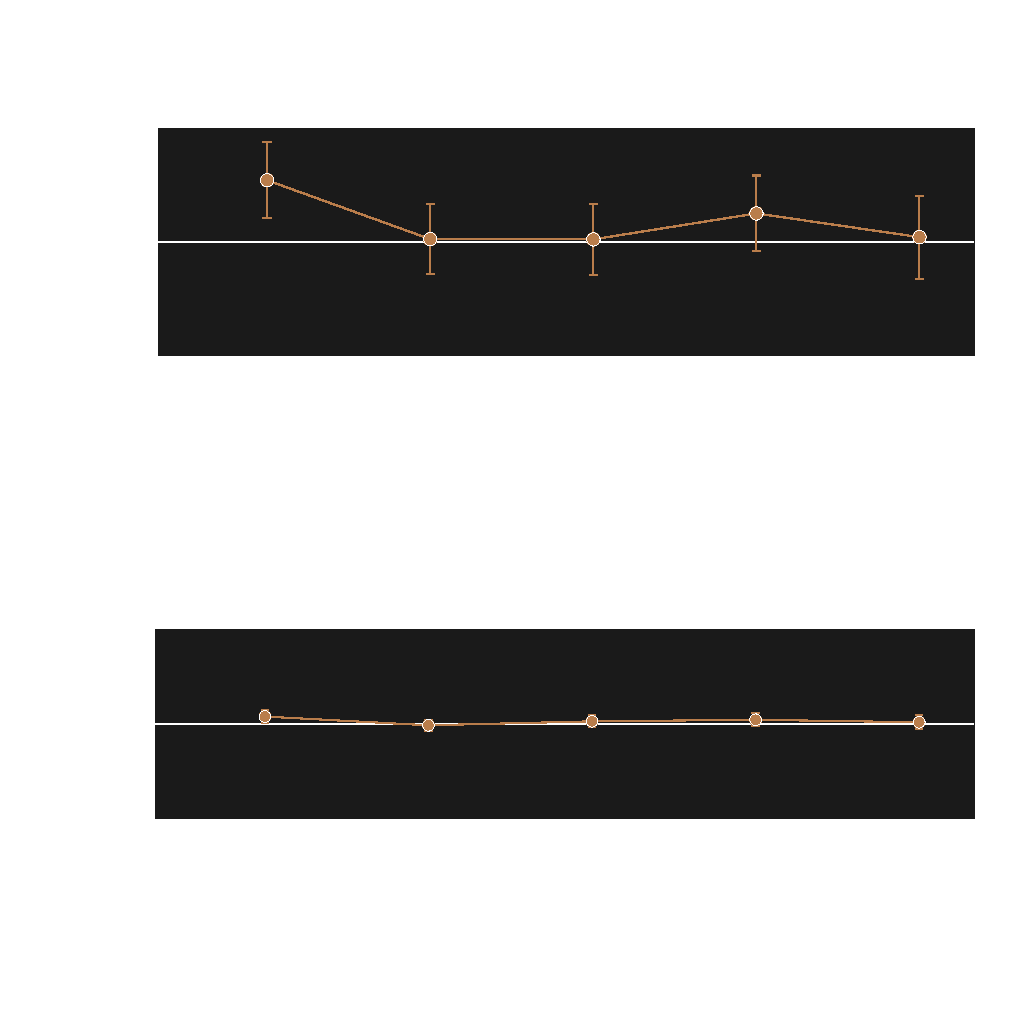
\includegraphics[width=\textwidth]{mc-select-bias-thresh-inv.pdf}
                \newline
            \end{center}
        \end{column}
    \end{columns}


}


\frame
{
    \frametitle{Too Close for Comfort?  Metacal Don't Care... \\But We Do}
 
    \begin{center}
        %\includegraphics[width=0.7\textwidth]{DES0428-4748_gri_crop.jpg}
        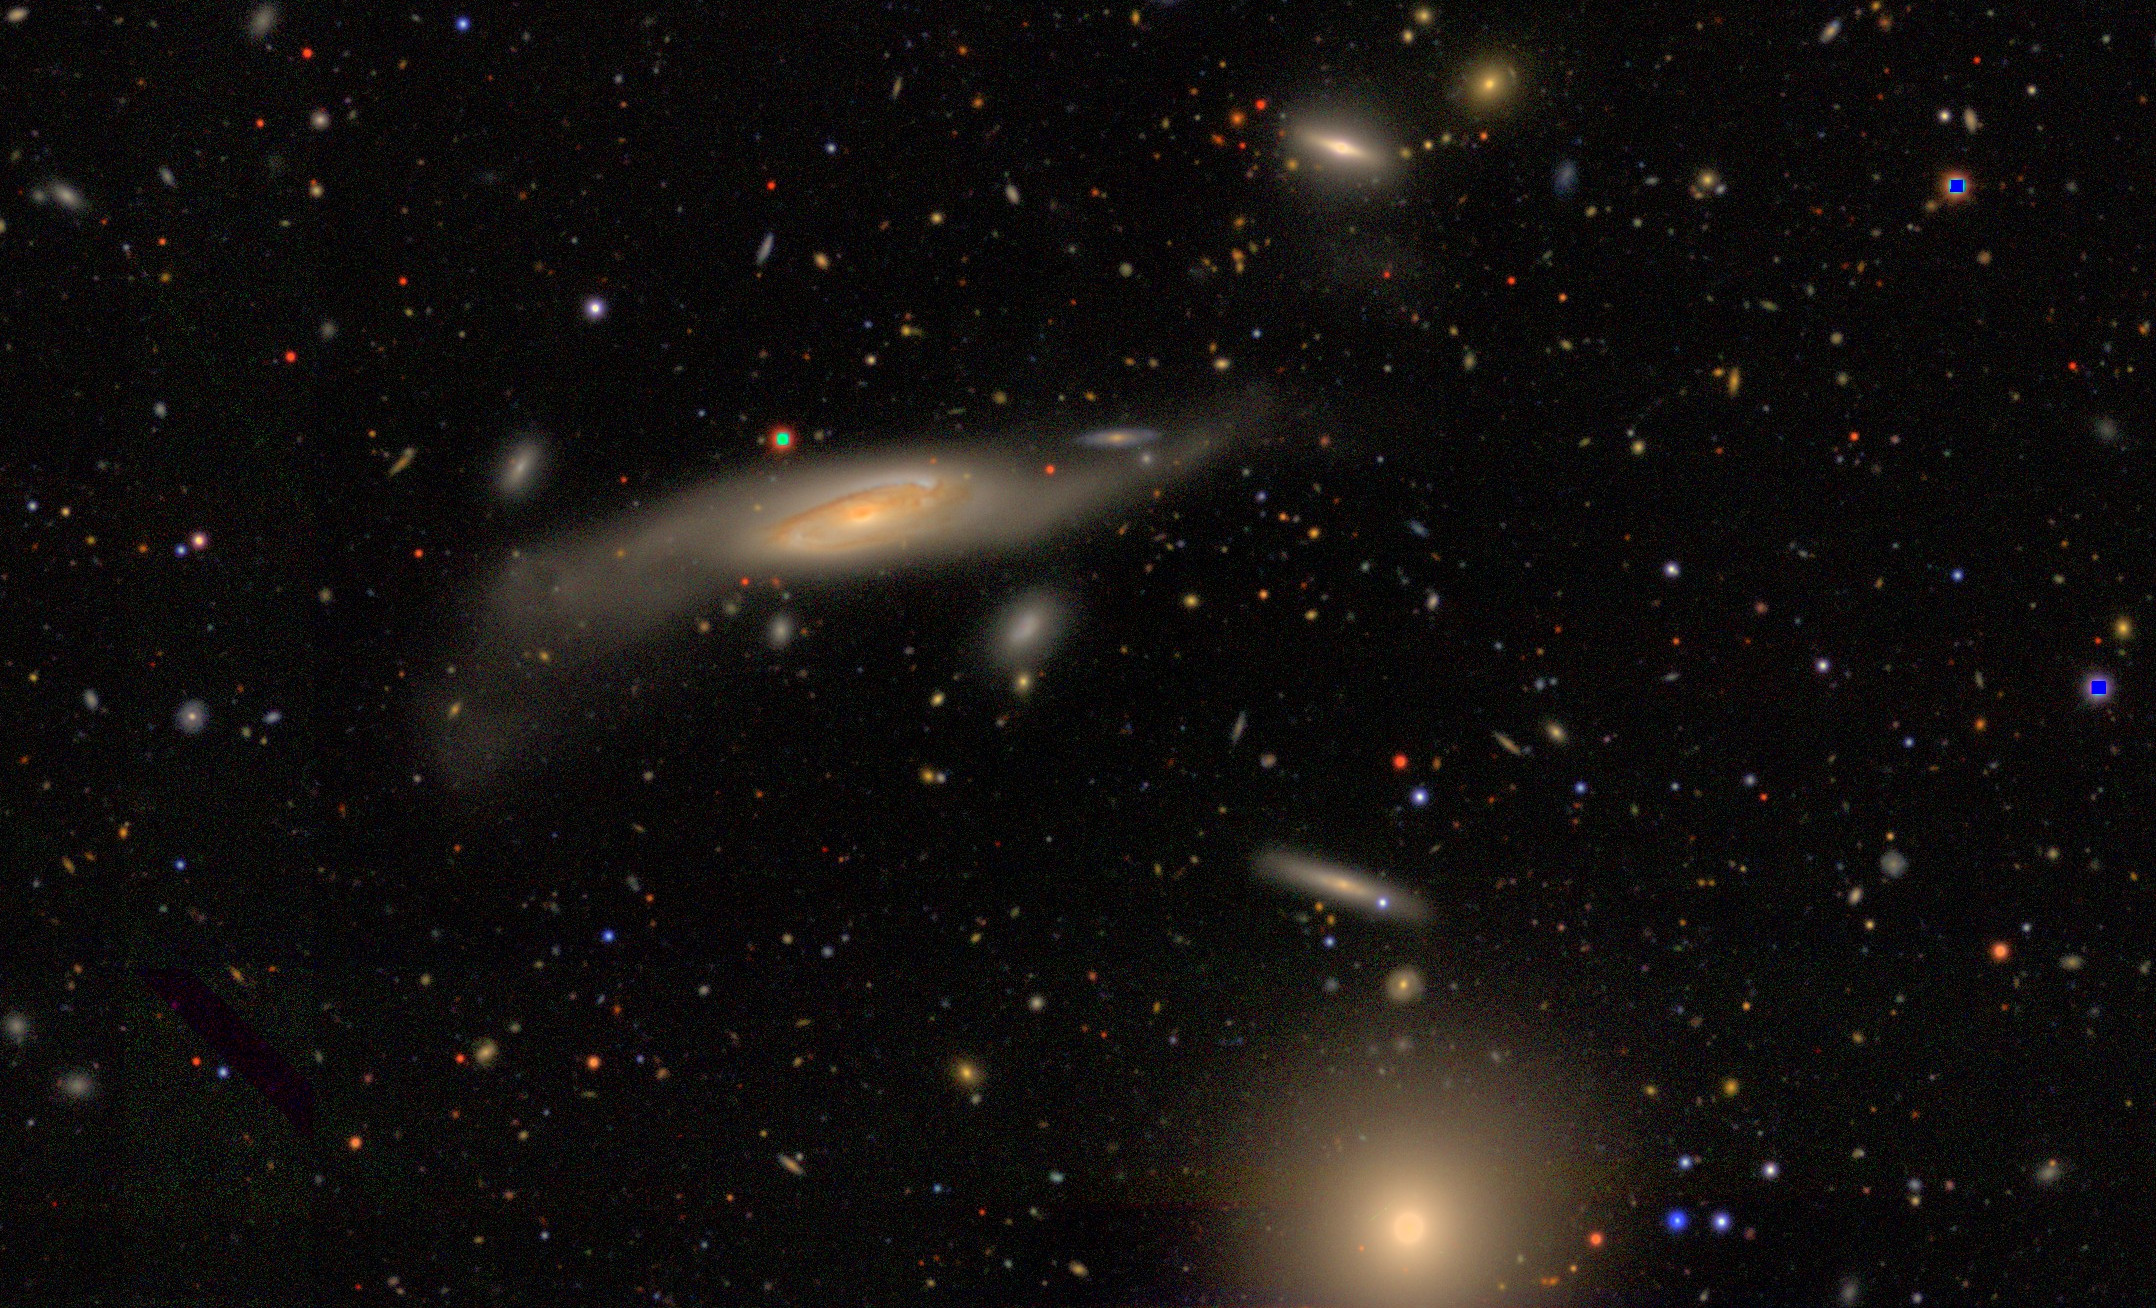
\includegraphics[width=0.9\textwidth]{DES0056-5248_gri_crop.jpg}
    \end{center}
    {\footnotesize Dark Energy Survey Image (Erin Sheldon)}

}

\frame
{
    \frametitle{Too Close for Comfort?  Metacal Don't Care... \\But We Do}
 
    \setbeamerfont*{itemize/enumerate body}{size=\normalsize}
    \setbeamerfont*{itemize/enumerate subbody}{parent=itemize/enumerate body}
    \setbeamerfont*{itemize/enumerate subsubbody}{parent=itemize/enumerate body}
 
    \begin{columns}
        \begin{column}{0.5\textwidth}
            \begin{itemize}
                \item \mcal\ will calculate the correct response
                    for blended objects.
                \item Good enough if they are at the same redshift
                \item If they are at different redshifts, then must
                    identify unique objects and separately
                    determine their redshifts and \mcal\ responses.
            \end{itemize}
        \end{column}
        \begin{column}{0.5\textwidth}
            \begin{center}
                %\includegraphics[width=\textwidth]{DES0428-4748_gri_crop.jpg}
                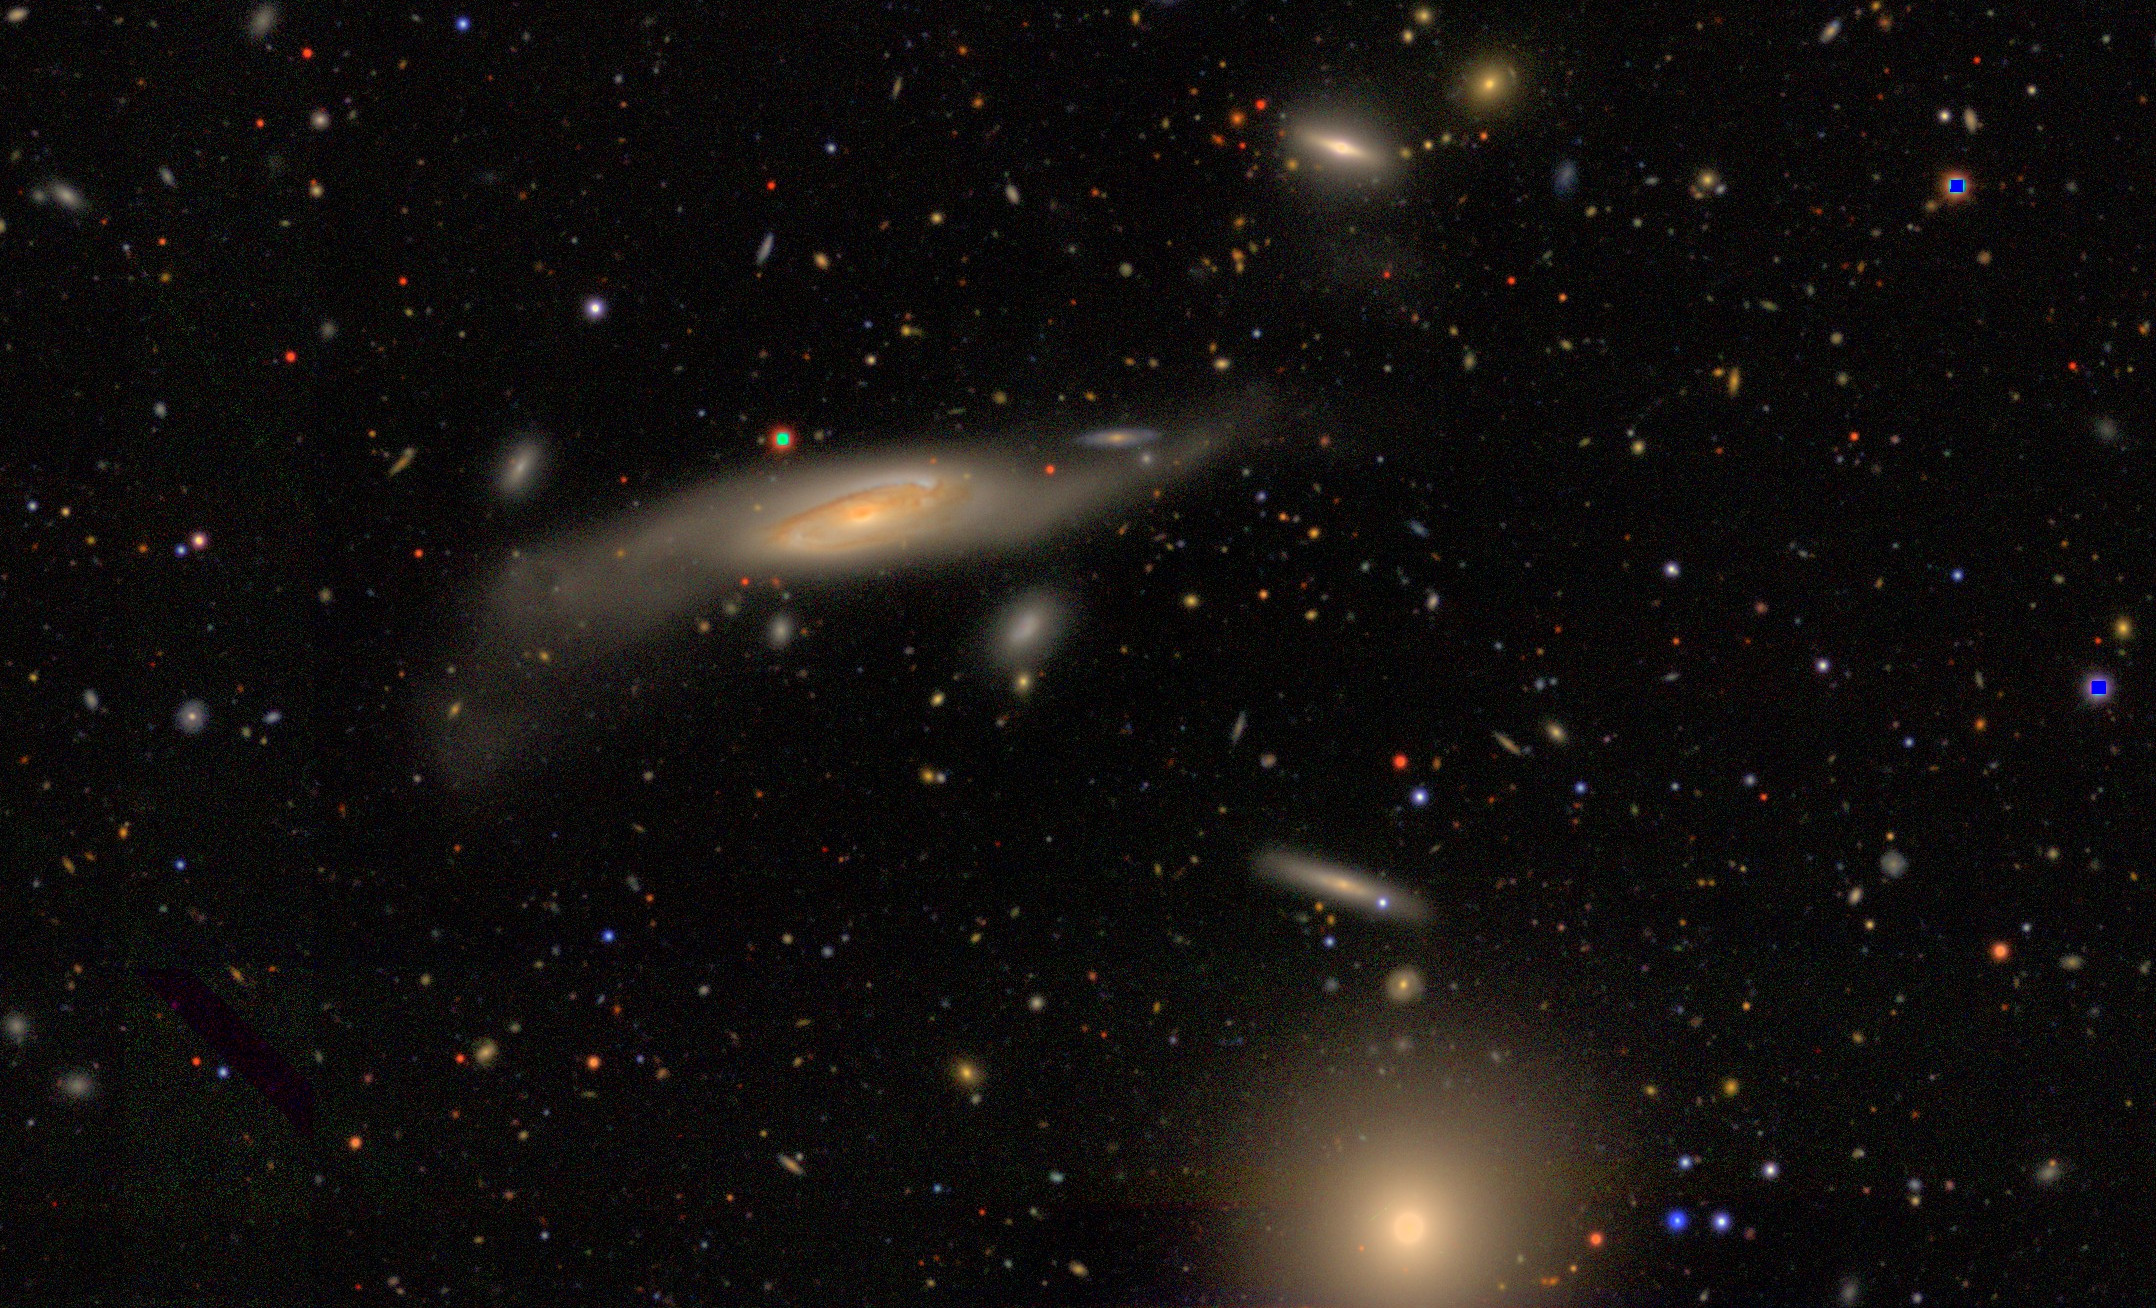
\includegraphics[width=\textwidth, angle=90]{DES0056-5248_gri_crop.jpg}
            \end{center}
                {\footnotesize Dark Energy Survey Image (Erin Sheldon)}
        \end{column}
    \end{columns}


}


\frame
{

    \frametitle{Simulation for Deblending Tests}


    \begin{itemize}
        \item Galaxy models same as previous simulations
        \item ``fake'' a fainter sample to mag 27.5 by scaling
            the flux and size of 25.2 sample.  Also fake extra bright galaxies.
        \item Half galaxies get shear 0.01, half get 0.02
        \item Place galaxies randomly on images mimicking DES coadds
        \item Add noise to achieve DES 5-year depth in $i$ band of 24.1
        \item Run through SExtractor, make MEDS files (Jarvis et al. 2016)

        \item Run \mcal\ in two modes, and attempt to recover mean
            shear for objects matched to input catalog.

    \end{itemize}


}

\frame
{
    \frametitle{Simulation for Deblending Tests }
 
    \begin{center}
        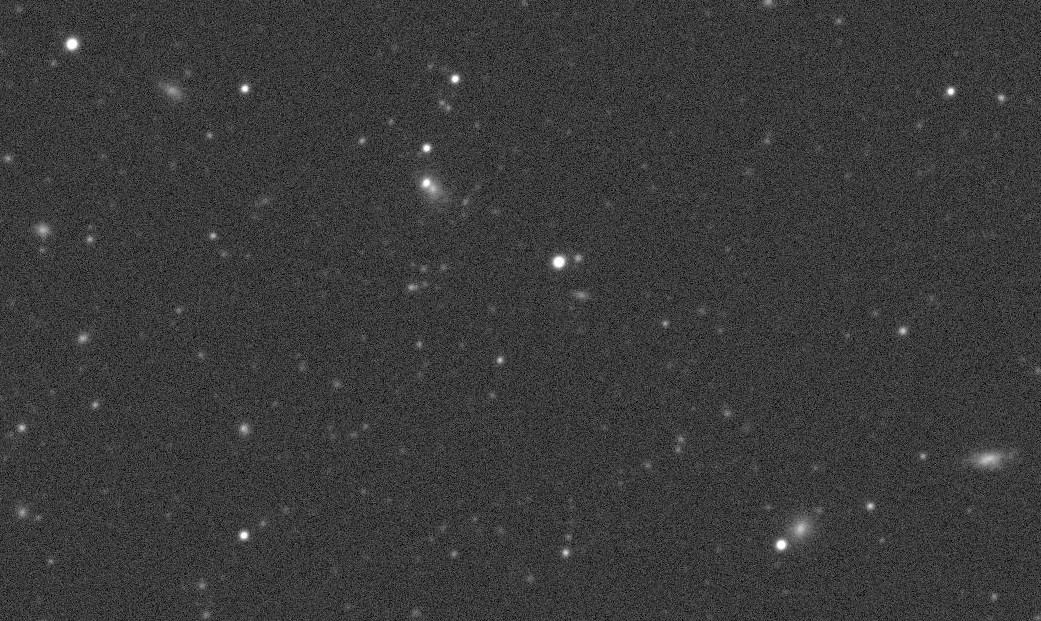
\includegraphics[width=\columnwidth]{nbrsim-003f-009969-image-crop.jpg}
    \end{center}

}


\frame
{

    \frametitle{Results for Deblending Tests}


    \begin{itemize}

        \item Run in two modes
        \item Mask neighbors using \uberseg\ algorithm (Jarvis et al. 2016)
            \begin{itemize}
                \item Use pixels closer to this object than any other.
                \item Don't use pixels assigned to another
                    object in the SExtractor segmentation map
            \end{itemize}

        \item Subtract the light from neighbors using the multi-object
            fitting (MOF: Matt Becker, Erin Sheldon)
            \begin{itemize}
                \item Fit blended objects semi-simultaneously (I can give details)
                \item https://github.com/esheldon/ngmix
                \item https://github.com/esheldon/ngmixer
            \end{itemize}


    \end{itemize}


}

\frame
{

    \frametitle{Results for Deblending Tests}

\begin{table}
    \centering
    \begin{tabular}{|l|c|c|c|}
        \hline
        Method         & \snr\ Cut & m            & c            \\
                       &           & $[10^{-2}]$  & $[10^{-5}]$  \\
        \hline

		\hline
        \uberseg       & \snr$ > 10$ & $+0.5 \pm 0.2$  & $-3.8 \pm 2.9$ \\
        \uberseg       & \snr$ > 15$ & $-0.0 \pm 0.2$  & $-4.4 \pm 3.1$ \\
        \uberseg       & \snr$ > 20$ & $+0.1 \pm 0.2$  & $-5.3 \pm 3.5$ \\

        \hline
        \uberseg+MOF   & \snr$ > 10$ & $-1.3 \pm 0.3$ & $-7.1 \pm 4.1$ \\
        \uberseg+MOF   & \snr$ > 15$ & $-1.7 \pm 0.3$ & $-6.3 \pm 4.3$ \\
        \uberseg+MOF   & \snr$ > 20$ & $-1.6 \pm 0.3$ & $-3.6 \pm 4.9$ \\


		\hline
    \end{tabular}
    \caption{Tentative detection of bias for \uberseg\ at \snr$>10$.
    Bias disappears with higher \snr\ cut.
    Clear detection of bias with \uberseg+MOF.
     \label{tab:mcal:deblending}}
\end{table}


}

\frame
{

    \frametitle{Promising New Deblender}

    \setbeamerfont*{itemize/enumerate body}{size=\Large}
    \setbeamerfont*{itemize/enumerate subbody}{parent=itemize/enumerate body}
    \setbeamerfont*{itemize/enumerate subsubbody}{parent=itemize/enumerate body}
 

    \begin{itemize}

        \item Melchior and Moolekamp working on a new
            deblender

        \item Minimal assumptions
            \begin{itemize}
                \item Object profiles decrease monotonically from peak
                \item Objects are symmetric under a 180 degree rotation
                \item Objects have no color gradients
            \end{itemize}

        \item In early stages but already works pretty well.
    \end{itemize}


}


\frame
{
    \frametitle{Example Deblend}
 
    \begin{center}
        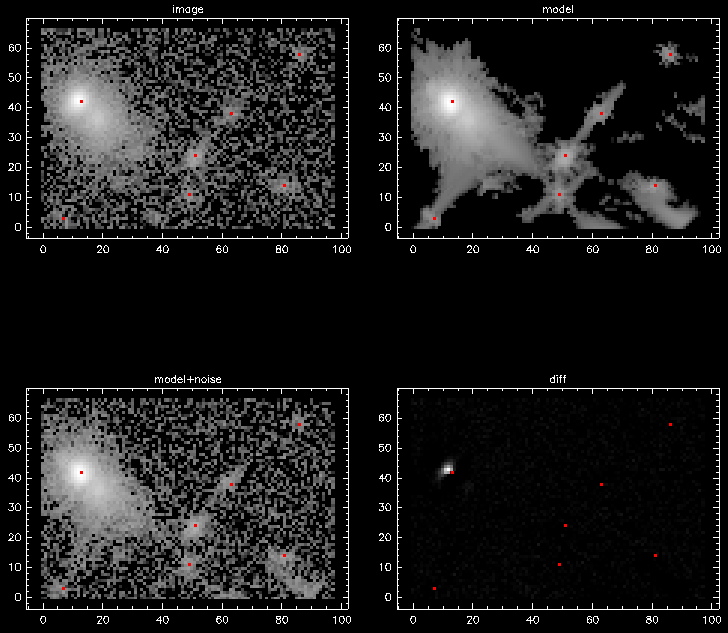
\includegraphics[width=0.8\textwidth]{nbrsim-003f-009969-modelcomp-sub000006-crop.png}
        \newline
    \end{center}

}




\frame
{
    \frametitle{Summary}
    \begin{itemize}
        \item \Mcal\ is a new method for shear measurement.
            \begin{itemize}
                \item Does not require significant prior knowledge about galaxy properties.
                \item Correct for noise bias, model bias, and selection effects within 
                    the formalism.

                \item In challenging simulations, recover shear to accuracy required
                    for LSST

                \item Relatively insensitive to the effects of neighbors.

            \end{itemize}

        \item Using \mcal\ for shear measurement in the Dark Energy Survey.

    \end{itemize}
}




\end{document}
